\chapter{Conclusion}

In this work, we developed a data-driven solution to find the best algorithm (here: linkage strategy) for clustering tasks on a given dataset. In section \ref{chapter:alphalinkage} we introduced an algorithm to efficiently interpolate between the in section \ref{chapter:relatedwork} described linkage strategies. The final $\alpha$-linkage algorithm uses a line sweep approach to find the pairwise distance function that leads to merges with the lowest resulting cost, i.e.\ the optimal clusterings.\\

While the in section \ref{chapter:relatedwork} described approaches are less efficient, our approach is able to analyze large parts of the in section \ref{chapter:setup}  discussed real-world datasets using cloud computing. We take multiple key observations from the experiments in section \ref{sec:results}:
\begin{itemize}
\item Interpolating between single and complete linkage overcomes the hurdles of clustering data where both single and complete linkage perform better for some certain parts of the data. While single and complete linkage lead to an error of approximately $25\%$ for our synthetic data, in some experiments $\alpha$-linkage leads to optimal clusterings.
\item For all our real-world datasets, we can sort the linkage strategies according to the quality in following order (best first):
\begin{enumerate}
\item Complete Linkage
\item Average Linkage
\item Single Linkage
\end{enumerate}
\item Interpolating between single and average linkage does in general not lead to significant improvements.
\item When interpolating between single and complete or average and complete linkage, $\alpha$-linkage outperforms the used linkage strategies in all of our experiments.
\item Parameter Advising is a very powerful tool to provide more accurate clusterings. Our greedy implementation allows to calculate the optimal parameter in an approximately optimal way very efficiently.
\end{itemize}

To be more precise, we show the results for the different datasets. In table \ref{table:comparison} we compare the single to complete linkage interpolation for all the discussed datasets\footnote{CIFAR 100 single to complete linkage was not discussed in section \ref{sec:results}.} in the batch setting. We notice that we achieve major improvements for all datasets and, excluding the synthetic data, receive similar values for $\alpha_{opt}$. This knowledge may be useful for transfer learning between different datasets in future work.

\begin{table}[H]
    \centering
    \begin{tabular}{|l | l | l | l | l | l |}
    \hline
    & Synthetic & NELL & MNIST & Omniglot & CIFAR10\\ \hline
    $\alpha_{opt}$ & 0.169 & 0.918 & 0.857 & 0.908 & 0.917\\
    $\Delta_{cost}$ & 22.70\% & 1.20\% & 3.70\% & 1.0\% & 0.2\%\\\hline
    \end{tabular}
    \caption{Comparing the results over the different datasets while interpolating between single and complete linkage leads to similar parameters for many datasets.}
    \label{table:comparison}
\end{table}

Similar to table \ref{table:comparison}, we also show the results for interpolating between average and complete linkage in table \ref{table:comparison_ac}.

\begin{table}[H]
    \centering
    \begin{tabular}{|l | l | l | l | l | l | l |}
    \hline
    & Synthetic & NELL & MNIST & Omniglot & CIFAR10 & CIFAR100\\ \hline
    $\alpha_{opt}$ & 0.201 & 0.855 & 0.633 & 0.798 & 0.539 & 0.875\\
    $\Delta_{cost}$ & 0.29\% & 0.77\% & 3.30\% & 1.0\% & 0.83\% & 1.8\%\\\hline
    \end{tabular}
    \caption{Comparing the results over the different datasets leads to a large spread of the parameters.}
    \label{table:comparison_ac}
\end{table}

In comparison to interpolating between single and complete linkage, we also get good improvements, however the optimal parameter $\alpha$ is spread more widely, i.e.\ it will be more difficult to reuse the gained knowledge for further use.\\

As we had implemented a framework to efficiently interpolate between inter-cluster distances, we also adapted it to interpolate between point distances in section \ref{sec:beta}. We generated image features with Convolutional Neural Networks and text features with Word Embeddings and showed in section \ref{sec:results} that we outperform all used feature representations.

\paragraph{Future Work.} Nevertheless we can think of further additions to this work. The trivial next step will be to combine metric learning with algorithm selection, as for now, we only evaluated the same setups independently, i.e.\ we used a static feature representation for algorithm selection and we used complete linkage for metric learning. At the point of writing this work, we are not exactly sure how difficult it will be to efficiently combine both aspects of this work, but we know that it is feasible and can be achieved in future work.\\

The proposed algorithms only work for linear interpolation between two algorithms. In this setting, proving that in each interval we perform the same optimal merge is mostly trivial. As an adaption of our algorithms, we can think of interpolating between more algorithms, e.g.\ we could interpolate between single, average and complete linkage with a distance such as the following:

\begin{align*}
&\mathcal{D}_\text{SAC}(X,Y) = \alpha_1 \cdot \min\limits_{x \in X, y \in Y} d(x,y) + \alpha_2 \cdot \frac{1}{|X||Y|} \sum\limits_{x \in X, y \in Y} d(x,y) + (1-\alpha_1-\alpha_2) \cdot \max\limits_{x \in X, y \in Y} d(x,y)\\
&\text{s. t. } \{\alpha_1, \alpha_2\} \in [0,1] \text{ and } \alpha_1 + \alpha_2 \le 1
\end{align*}

However, the distance functions $d_{(\alpha_1, \alpha_2)}$ now are not linear anymore, as they depend on the two parameters $\alpha_1$ and $\alpha_2$. This means that our suggested line sweep approach will not work anymore, as the distance depending on the two parameter spans a three-dimensional space, where each split is a convex hull instead of a linear subspace. Figure \ref{fig:convexhull} shows the interval split depending on $\alpha$ on the left, and the split depending on $\alpha_1$ and $\alpha_2$ on the right. Our example shows a very optimistic example where the splitting linear functions are parallel, however this might often not be the case, i.e.\ we will receive more different regions where it will be less intuitive to find the borders where and when one merge is preferred over another (e.g.\ see figure \ref{fig:convexhulls2}).

\begin{figure}[h]
\centering
\begin{minipage}{.45\textwidth}
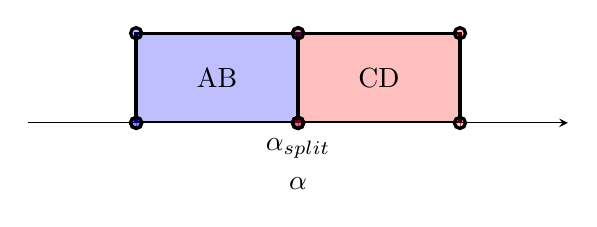
\begin{tikzpicture}
\begin{axis}[
    xmin=0, xmax=1,
    axis x line=bottom,% only show the bottom x axis
    xlabel={$\alpha$},
    xtick={0.2,0.5,0.8},
    xticklabels={$\alo$,$\alpha_{split}$,$\ahi$},
    hide y axis,    
    ymin=0,ymax=5,
    scatter/classes={%
        a={mark=o,draw=black}}
    ]

    \addplot [mark=*,very thick,fill=blue, fill opacity=0.25] coordinates {
        (0.2, 0)
        (0.2, 1)
        (0.5, 1)
        (0.5, 0)
        (0.2, 0)
    };
    \addplot [mark=*,very thick,fill=red, fill opacity=0.25] coordinates {
        (0.5, 0)
        (0.5, 1)
        (0.8, 1)
        (0.8, 0)
        (0.5, 0)
    };
    \node[] at (axis cs: 0.35,0.5) {AB};
    \node[] at (axis cs: 0.65,0.5) {CD};
\end{axis}
\end{tikzpicture}
\end{minipage}
\begin{minipage}{.45\textwidth}
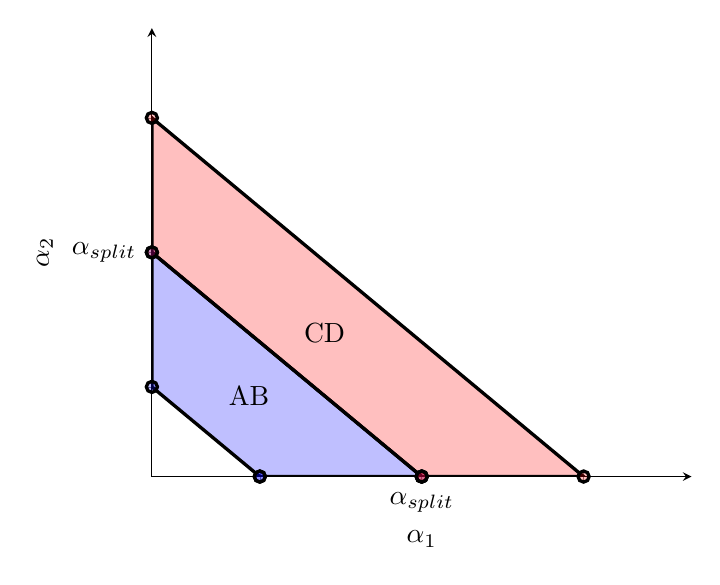
\begin{tikzpicture}
\begin{axis}[
    xmin=0, xmax=1,
    axis x line=bottom,% only show the bottom x axis
    axis y line=left,
    xlabel={$\alpha_1$},
    ylabel={$\alpha_2$},
    xtick={0.2,0.5,0.8},
    xticklabels={$\alo$,$\alpha_{split}$,$\ahi$},  
    ytick={0.2,0.5,0.8},
    yticklabels={$\alo$,$\alpha_{split}$,$\ahi$},  
    ymin=0,ymax=1,
    scatter/classes={%
        a={mark=o,draw=black}}
    ]

    \addplot [mark=*,very thick,fill=blue, fill opacity=0.25] coordinates {
        (0.2, 0)
        (0.5, 0)
        (0, 0.5)
        (0, 0.2)
        (0.2, 0)
    };
    \addplot [mark=*,very thick,fill=red, fill opacity=0.25] coordinates {
        (0.5, 0)
        (0.8, 0)
        (0, 0.8)
        (0, 0.5)
        (0.5, 0)
    };
    \node[] at (axis cs: 0.18,0.18) {AB};
    \node[] at (axis cs: 0.32,0.32) {CD};
\end{axis}
\end{tikzpicture}
\end{minipage}
\caption{While in this work, the split between different merges was based on a linear function $d(\alpha)$ (left), it will be more difficult to evaluate the merges when interpolating with two weight parameters $\alpha_1$ and $\alpha_2$, where the merges will be represented as a convex hull in the $\alpha_1$-$\alpha_2$-space (right).}
\label{fig:convexhull}
\end{figure}

\begin{figure}[h]
\centering
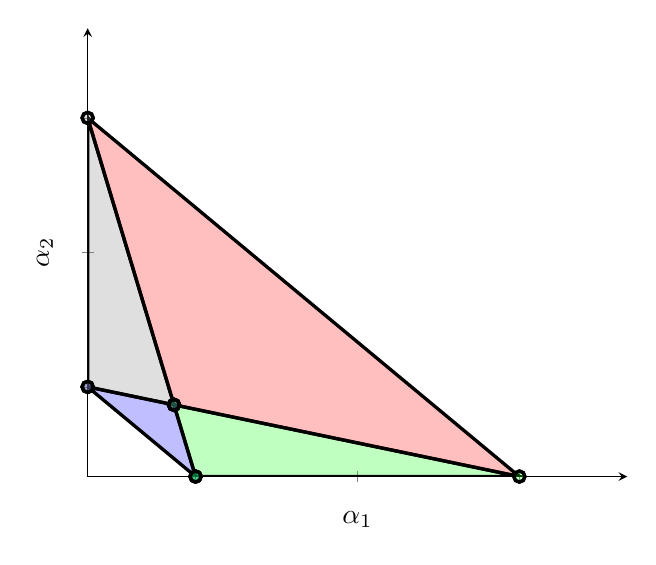
\begin{tikzpicture}
\begin{axis}[
    xmin=0, xmax=1,
    axis x line=bottom,% only show the bottom x axis
    axis y line=left,
    xlabel={$\alpha_1$},
    ylabel={$\alpha_2$},
    xtick={0.2,0.5,0.8},
    xticklabels={$\alo$,,$\ahi$},  
    ytick={0.2,0.5,0.8},
    yticklabels={$\alo$,,$\ahi$},  
    ymin=0,ymax=1,
    scatter/classes={%
        a={mark=o,draw=black}}
    ]
    \addplot [mark=*,very thick,fill=blue, fill opacity=0.25] coordinates {
        (0.2, 0)
        (0, 0.2)
        (0.16, 0.16)
        (0.2, 0)
    };
    \addplot [mark=*,very thick,fill=green, fill opacity=0.25] coordinates {
        (0.2, 0)
        (0.8, 0)
        (0.16, 0.16)
        (0.2, 0)
    };
    \addplot [mark=*,very thick,fill=gray, fill opacity=0.25] coordinates {
        (0, 0.2)
        (0, 0.8)
        (0.16, 0.16)
        (0, 0.2)
    };
    \addplot [mark=o,very thick,fill=red, fill opacity=0.25] coordinates {
        (0.16, 0.16)
        (0.8, 0)
        (0, 0.8)
        (0.16, 0.16)
    };
\end{axis}
\end{tikzpicture}
\caption{Finding the merges in the different regions can be more challenging when interpolating with two weight parameters $\alpha_1$ and $\alpha_2$.}
\label{fig:convexhulls2}
\end{figure}

In addition, we can apply the introduced algorithm to more datasets and data domains, such as the sets contained in the UCI Machine Learning Repository \cite{Dua:2019}. For instance, we could compare different datasets within one specific data domain. Say we evaluate a variety of different image datasets and compare the optimal values of $\alpha$. An interesting observation would be, if we could reuse the optimal parameter from different datasets within the same or even across other domains. In our experiments, we often found similar optimal values in the range $[0.7,0.9]$ while other ranges mostly did not lead to good results (e.g.\ $[0.0, 0.5]$). We could use this knowledge for further experiments by e.g. evaluating only smaller regions or by putting more emphasis on given parameters in general. We can then also evaluate other domains, such as (partially) labeled voice datasets and compare the results across different data domains.\\

Also, we can imagine applying this framework to (a) other clustering algorithms than agglomerative hierarchical clustering and (b) other tasks than clustering.